\documentclass{letask}

\begin{document}
\begin{titlepage}
\center % Center everything on the page
 
%----------------------------------------------------------------------------------------
%	HEADING SECTIONS
%----------------------------------------------------------------------------------------

\textsc{\LARGE Московский\\[-0.2cm]Физико-Технический Институт\\[0.1cm]\large (государственный университет)}\\[1.5cm] % Name of your university/college
\textsc{\Large Кафедра общей физики}\\[0.1cm] % Major heading such as course name
\textsc{\large Лабораторная работа \textnumero  4.5.2}\\[0.5cm] % Minor heading such as course title

%----------------------------------------------------------------------------------------
%	TITLE SECTION
%----------------------------------------------------------------------------------------

\HRule
\\[0.4cm]
{ \huge \bfseries Интерференция\\[0.2cm]
лазерного излучения}
\\[0.6cm] % Title of your document
\HRule
\\[1.5cm]


 
%----------------------------------------------------------------------------------------
%	AUTHOR SECTION
%----------------------------------------------------------------------------------------


	\begin{flushleft} \large
		\textsf{Студент}
		
		Северилов Павел \\[-0.15cm]
		671 группа
	\end{flushleft}


\begin{bottompar}
	\begin{center}
		
\includegraphics[width = 80 mm]{logo.jpg}
	\end{center}
	{\large \today}

\end{bottompar}
\vfill % Fill the rest of the page with whitespace

\end{titlepage}

\textbf{Цель работы:} исследовать зависимость видности интерференционной картины от разности хода интерферирующих лучей и от их поляризации.

\textbf{В работе используются:} гелий-неоновый лазер, интерферометр Майкельсона с подвижным зеркалом, фотодиод с усилителем, осциллограф С1-76, поляроид, линейка.

\section{Теоретическая часть}

Лазер состоит из двух зеркал, составляющих лазерный резонатор, и расположенной между ними газообразной усиливающей среды, состоящей из гелия и неона. Характерное расстояние между зеркалами ~--~$0.2 \div 1 \m$. 

Излучение распространяется по резонатору в прямом и обратном направлениях. При этом максимальным усилением обладают волны, для которых набег фазы при полном обходе резонатора кратен $2 \pi$. Тогда можно сформулировать условие на разность частот излучения. Так как:
\[ \dfrac{2 \pi}{\lambda}2L = 2 \pi m,	\quad L=m\lambda, \quad \nu_{m}=\dfrac{mc}{2L}, \]
тогда:

\begin{equation}
\label{eq:cond}
\Delta \nu_{m}=\nu_{m+1}-\nu_{m}=\dfrac{c}{2L},
\end{equation}

где $L$ -- длина резонатора, $m$ -- целое число. Поэтому лазер генерирует отдельные типы колебаний, называемые модами, удовлетворяющие условию (\ref{eq:cond}). 

Спектральная ширина отдельной моды определяется добротностью резонатора лазера и мощностью излучения. В He-Ne лазере из-за малого усиления активной среды используются зеркала с высоким отражением. добротность резонатора большая и спектральная ширина моды может быть очень узкой, вплоть до единиц $\Hz$. Ввиду наличия тепловых флуктуаций длины резонатора типичная ширина моды составляет $10^5 \; \Hz$. Количество генерируемых мод определяется шириной спектра усиления активной среды. Эта ширина складывается из естественной ширины линии излучения атомов неона и доплеровского уширения, вызванного тепловым движением атомов. При температуре $400 \K$ ширина по полувысоте спектра излучения газообразного неона равна $1.5 \cdot 10^{9} \; \Hz$.

Вследствие тепловых флуктуаций длина резонатора меняется, в результате чего моды "переползают" с одного края контура на другой, там исчезают, а на другом краю рождаются новые. Таким образом температура нестабильность приводит к медленным изменениям амплитуд колебаний в лазерных модах и числа самих мод.

\begin{wrapfigure}[15]{L}{0.4 \lw}
	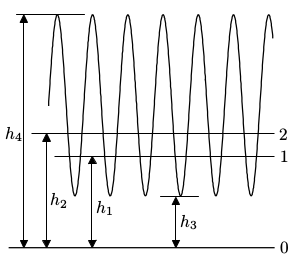
\includegraphics[width =  \lw]{img1}
	\caption{Осциллограмма сигналов фотодиода}
	\label{fig:somelabel}
\end{wrapfigure}

\textbf{Видность интерференционной картины.} Если в плоскости наблюдения две плоские волны с длиной волны $\lambda_{0}$ сходятся под малым углом $\alpha$, то наблюдается интерференционная картина в виде последовательности темных и светлых полос c расстоянием между ними:
\begin{equation}
\label{eq:deltax}
\Delta x = \dfrac{\lambda_{0}}{\alpha}
\end{equation}

Для оценки чёткости интерференционной картины в окрестности некоторой точки используют параметр видимости:
\begin{equation}
\label{eq:seen}
V=\dfrac{I_{max}-I_{min}}{I_{max}+I_{min}},
\end{equation}

где $I_{max}$ и $I_{min}$ -- максимальная и минимальная интенсивности света интерференционной картины вблизи выбранной точки. Человеческий глаз может уверенно различать чередование светлых и темных полос при $V \geq 0,1$. 

Пусть интерферируют две волны с амплитудами $A_{m}$ и $B_{m}$. Если в точке наблюдения разность фаз между волнами равна $k_{m} l$, где $k_{m}$ -- волновое число, $l$ -- разность хода, то интенсивность света в этой точке:
\begin{equation}
\label{eq:intensity}
I_{m} = {A_{m}}^2+{B_{m}}^2+2 A_{m} B_{m} cos(k_{m}l)
\end{equation} 
В максимуме интенсивность $I_{max} = (A_{m}+B_{m})^2$, в минимуме $I_{min} = (A_{m}-B_{m})^2.$ Отсюда видность:
\begin{equation}
\label{eq:seen1}
V_{1} = \dfrac{2 \sqrt{\delta}}{1+\delta},
\end{equation}
где $\delta = (B_{m}/A_{m})^2$.

Рассмотрим влияние спекрального состава на видность интерференционной картины:
\begin{equation}
V_{2}(l) = \dfrac{\sum_{n=1}^{\infty} {A_{n}}^2 cos(\dfrac{2 \pi \Delta \nu n l}{c})}{\sum_{n=1}^{\infty}{A_{n}}^2}.
\end{equation}

Введем также поправку к видности, связанную с углом между плоскостями поляризации падающих волн:
\begin{equation}
V_{3} = cos \beta,
\end{equation}
где $\beta$ -- угол между плоскостями поляризации.
Кроме того, по данным осциллограммы (рис.1) можно определить
\begin{equation}
\delta = \dfrac{h_{1}}{h_{2}}
\end{equation}

\begin{equation}
V = \dfrac{h_{4}-h_{3}}{h_{4}+h_{3}},
\end{equation}

где $V$ -- полная видимость. Если имеют место все три фактора уменьшения видимости: неравенство амплитуд, несовпадение поляризаций и разная оптическая задержка между интерферирующими пучками, то:
\begin{equation}
V = V_{1} \cdot V_{2} \cdot V_{3}.
\end{equation}	
	
\section{Экспериментальная установка}

\begin{figure}[H]
\centering
	\begin{center}
		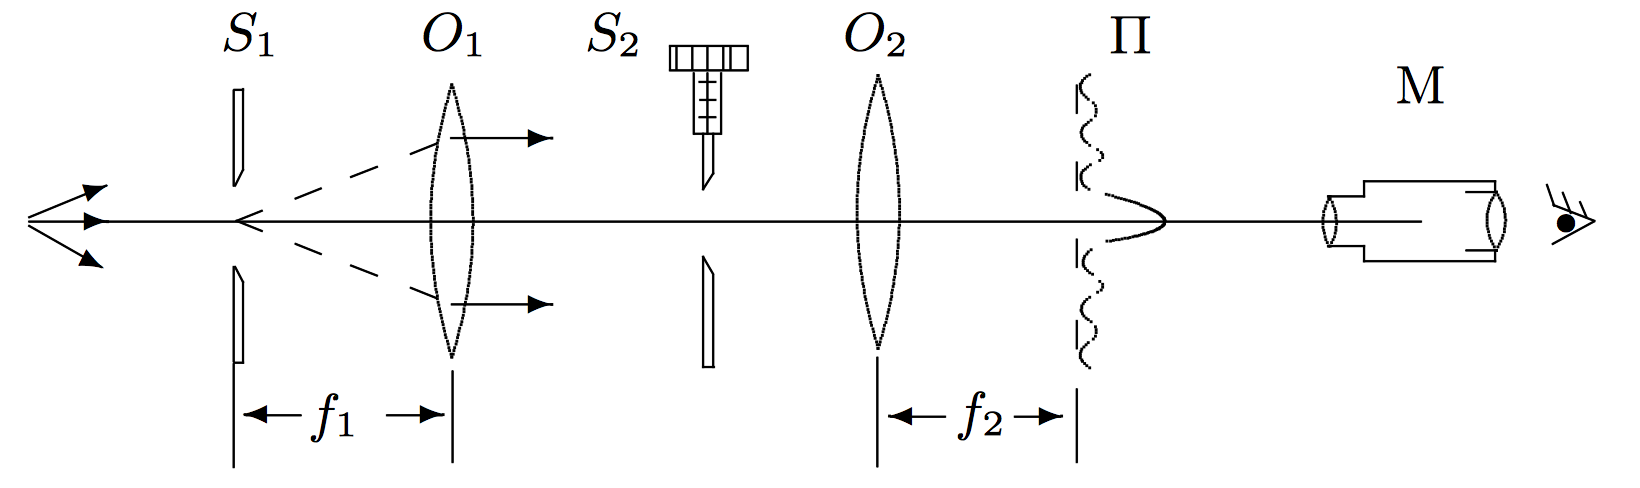
\includegraphics[width = 0.9 \lw]{img2}
	\end{center}
	\caption{Схема экспериментальной установки}
\end{figure}

Экспериментальная установка представляет собой интерферометр Майкельсона, смонтированный на вертикально стоящей плите. Источником света служит гелий-неоновый лазер ($\lambda_{0} = 632,8 \nm$). Пучок лазерного излучения отражается от зеркала З и проходит через ромб Френеля(РФ).

Пучок 1 проходит поляроид $\text{П}_{1}$, отражается под небольшим углом от зеркала $\text{З}_1$, снова проходит поляроид $\text{П}_{1}$ и, частично отражаясь от диагональной плоскости делительного кубика, выходит из интерферометра, попадая на зеркало $\text{З}_3$ и фотодиод ФД. При этом можно вращать $\text{П}_{1}$, изменяя плоскость поляризации.

Пучок 2 проходит линзу Л, поляроид $\text{П}_2$, отражается от зеркала $\text{З}_2$, снова проходит $\text{П}_{2}$, линзу Л и делительный кубик, выходит из интерферометра, попадает на зеркало $\text{З}_3$ и далее на фотодиод ФД. Таким образом, от зеркала $\text{З}_3$ под небольшим углом друг к другу идут на фотодиод два пучка, проходящие через разные плечи интерферометра. Для питания усилителя сигнала фотодиода и управления пьезокерамикой используется блок питания БП.


\section{Установка и параметры измерения}

Расстояние между зеркалами лазера: $65~\cm$.

\subsection*{Зависимость видности от угла $\beta$ поворота поляроида}


\begin{table}[H]
\centering
\caption{Измерим зависимость видности $\nu_3$ от угла поворота поляроида при нулевой разности хода}
\begin{tabular}{|c|c|c|c|c|c|c|c|c|c|c|}
\hline
$\beta, ~^\circ$ & $h_1$ & $h_2$ & $h_3$ & $h_4$ & $\delta$ & $\nu$ & $\nu_1$ & $\nu_3$ & $\cos \beta$ & ${\cos}^2 \beta$ \\ \hline
90	&0,2	&1		 &1		  &1,6	&0,200	&0,231	&0,745	&0,310	&0,000	&0,000	\\ \hline
80	&0,6	&5,4	&5,4	&6,6	&0,111	&0,100	&0,600	&0,167	&0,174	&0,030	\\ \hline
70	&0,5	&5,4	&5		 &7		&0,093	&0,167	&0,557	&0,299	&0,342	&0,117	\\ \hline
60	&0,4	&5,3	&4,8	&6,6	&0,075	&0,158	&0,511	&0,309	&0,500	&0,250	\\ \hline
50	&0,5	&5,2	&4,4	&7		&0,096	&0,228	&0,566	&0,403	&0,643	&0,413	\\ \hline
40	&0,9	&5,2	&4,1	&8		&0,173	&0,322	&0,709	&0,454	&0,766	&0,587	\\ \hline
30	&0,4	&2,1	&2,5	&6,6	&0,190	&0,451	&0,733	&0,614	&0,866	&0,750	\\ \hline
20	&0,6	&2,1	&1,2	&4,1	&0,286	&0,547	&0,831	&0,658	&0,940	&0,883	\\ \hline
15	&0,7	&2,1	&1,1	&5,6	&0,333	&0,672	&0,866	&0,776	&0,966	&0,933	\\ \hline
10	&0,6	&2,1	&1,1	&5,4	&0,286	&0,662	&0,831	&0,796	&0,985	&0,970	\\ \hline
5	&0,6	&2,2	&1		&5,6	&0,273	&0,697	&0,821	&0,849	&0,996	&0,992	\\ \hline
0	&0,9	&2,2	&1		&5,2	&0,409	&0,677	&0,908	&0,746	&1,000	&1,000           \\ \hline
\end{tabular}
\end{table}

\begin{figure}[H]
\centering
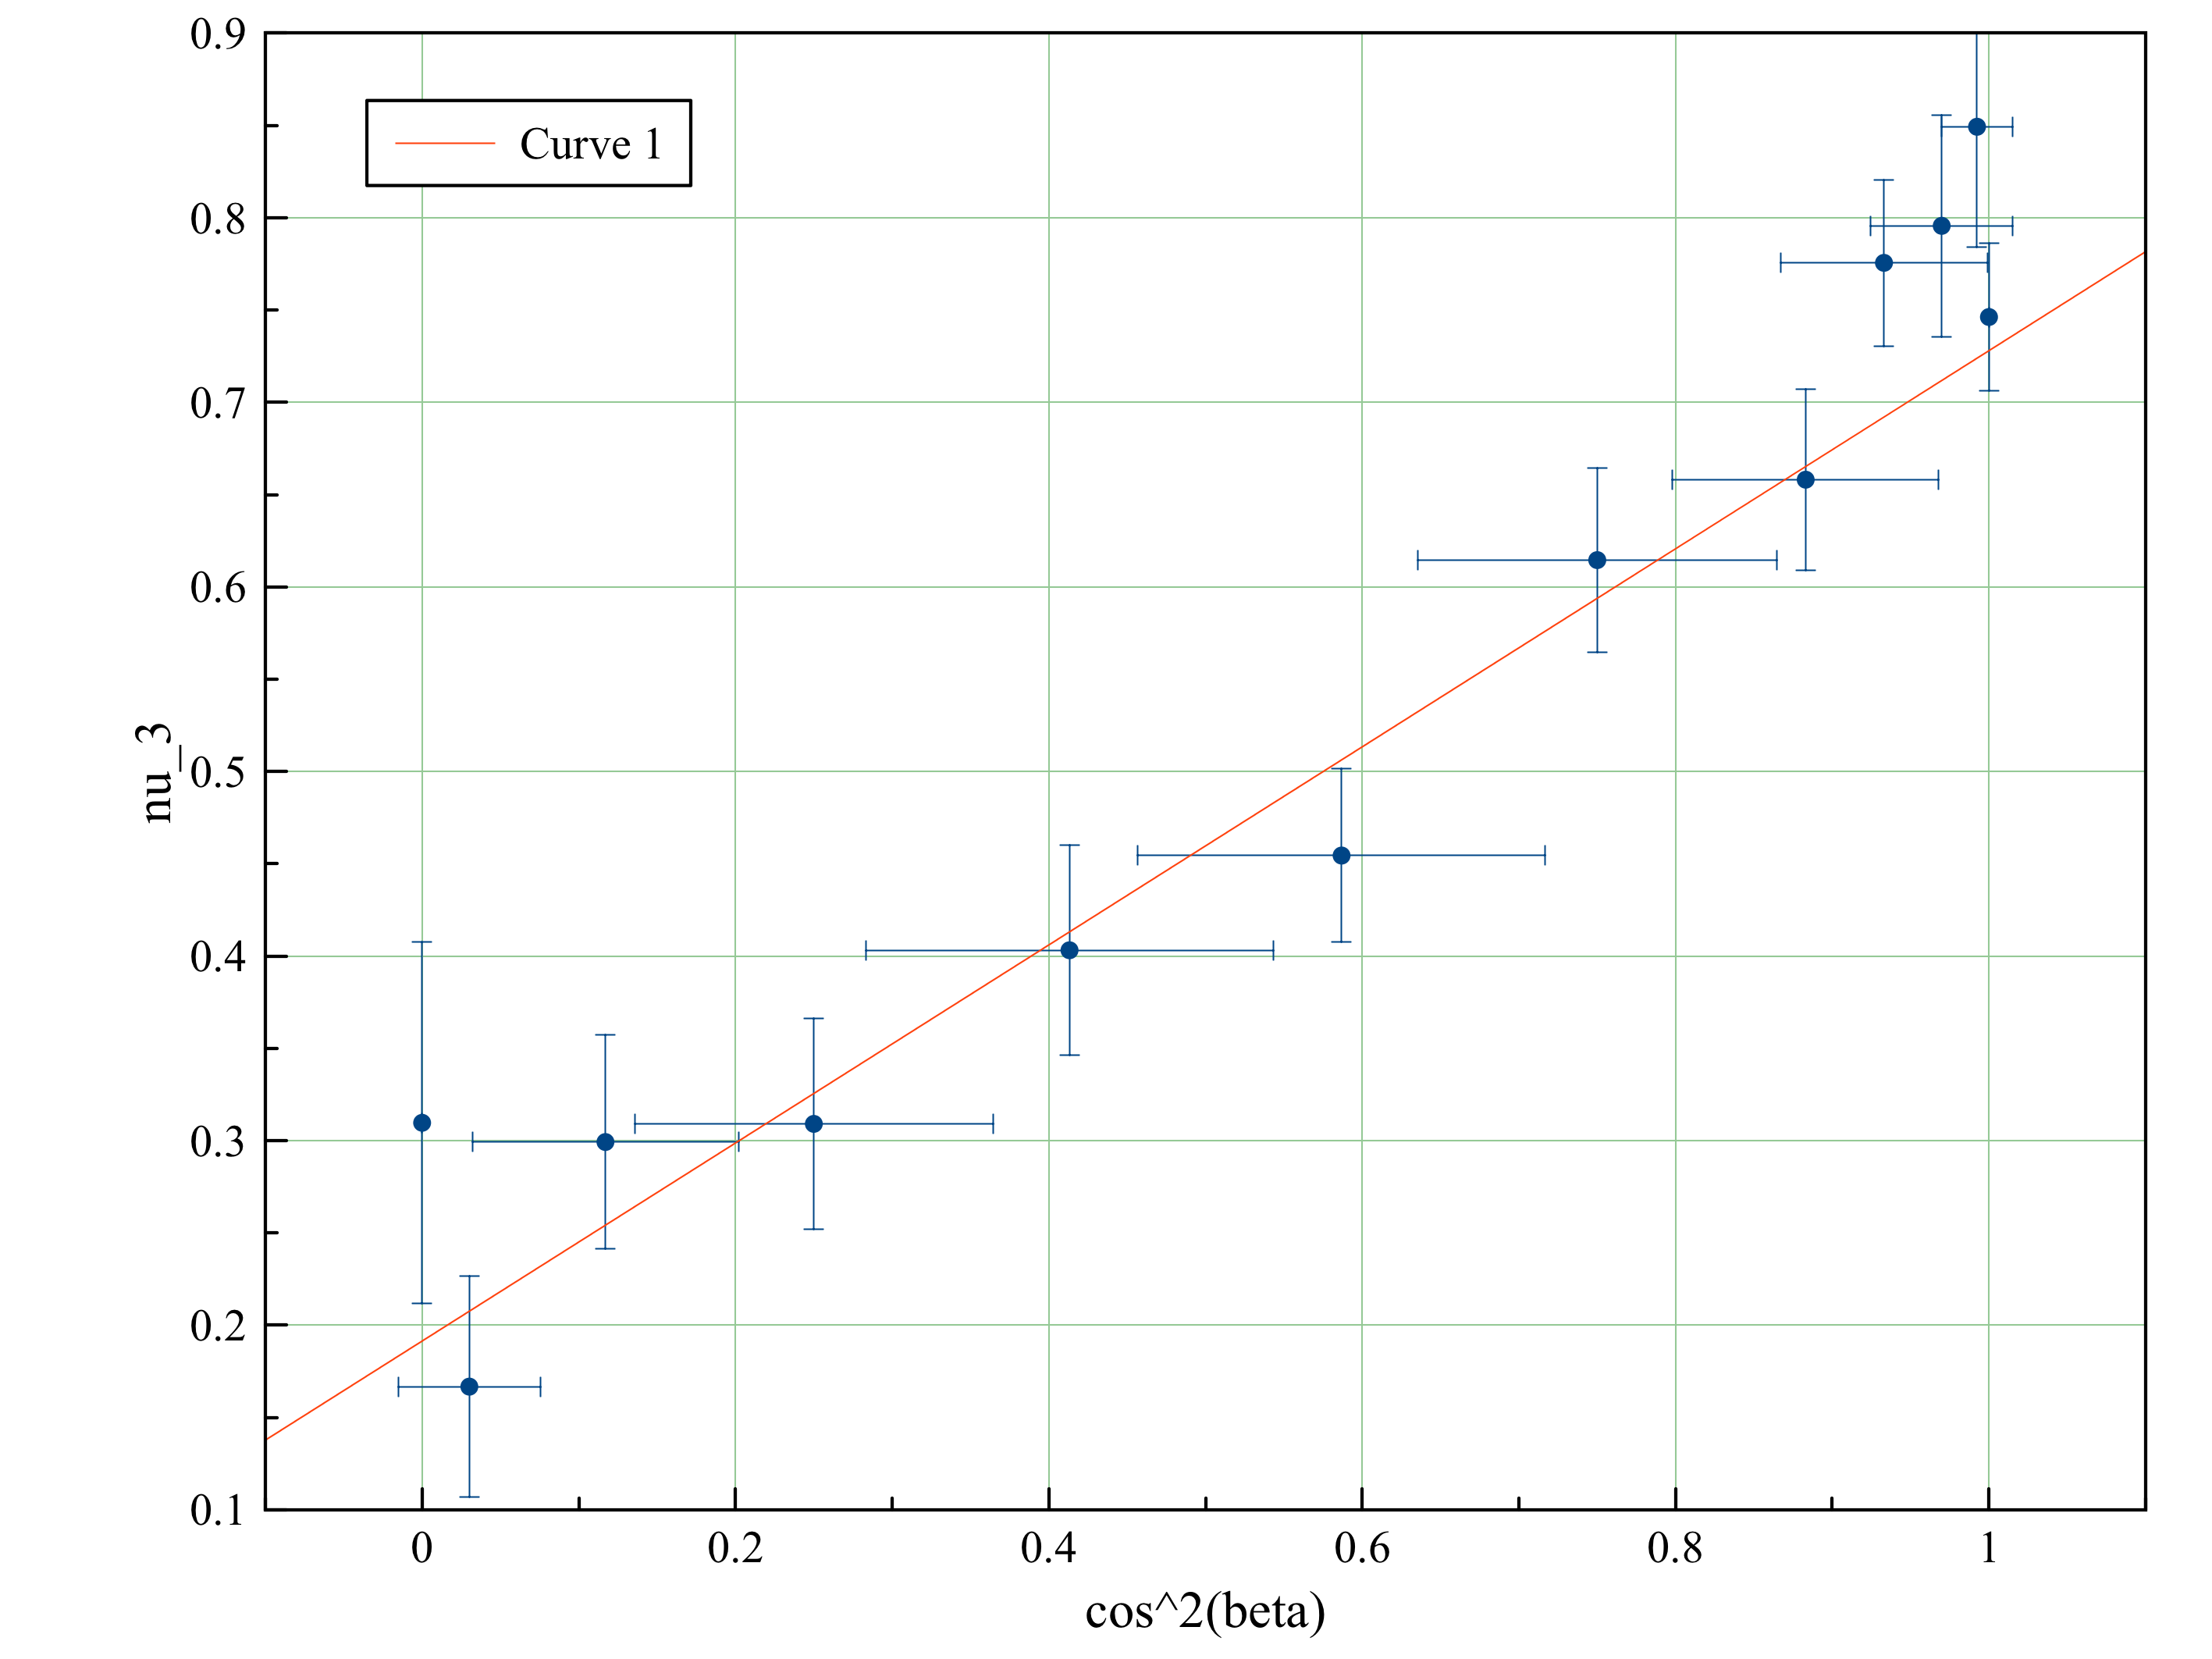
\includegraphics[width = 0.75 \lw]{1.png}
\caption{График зависимости $ \nu({\cos}^2 \beta) $}
\end{figure}


\subsection*{Зависимость видности $\nu_2$ от координаты $x$ блока}
\begin{table}[H]
\centering
\caption{Измерим зависимость видности $\nu_2$ от координаты $x$ блока}
\begin{tabular}{|c|c|c|c|c|c|c|c|c|}
\hline
$x$ & $h_1$ & $h_2$ & $h_3$ & $h_4$ & $\delta$ & $\nu$ & $\nu_1$ & $\nu_2$ \\ \hline
10&	0,9&	4&		2,8&	6,8&	0,225&	0,417&	0,774&	0,538\\ \hline
14&	0,85&	3,15&	2,0&	6,2&	0,270&	0,512&	0,818&	0,626\\ \hline
16&	0,4&	2,9&	2,6&	6,4&	0,138&	0,422&	0,653&	0,647\\ \hline
18&	0,9&	4,9&	3,1&	8,0&	0,184&	0,441&	0,724&	0,610\\ \hline
20&	2,3&	2,8&	1,8&	8,0&	0,821&	0,633&	0,995&	0,636\\ \hline
25&	2,3&	1,3&	2,6&	4,7&	0,565&	0,288&	0,961&	0,299\\ \hline
30&	4,7&	1,5&	5,6&	6,6&	0,319&	0,082&	0,857&	0,096\\ \hline
32&	4,5&	1,8&	5,8&	6,5&	0,400&	0,057&	0,904&	0,063\\ \hline
34&	4,5&	2,7&	6,8&	7,7&	0,600&	0,062&	0,968&	0,064\\ \hline
40&	2,4&	1,6&	3,4&	4,7&	0,667&	0,160&	0,980&	0,164\\ \hline
43&	0,9&	3,7&	4,2&	5,2&	0,243&	0,106&	0,793&	0,134\\ \hline
50&	2,2&	2,8&	4,8&	6,2&	0,786&	0,127&	0,993&	0,128\\ \hline
60&	2,2&	2,7&	4,6&	5,3&	0,815&	0,071&	0,995&	0,071\\ \hline
70&	2,2&	0,9&	2,9&	5,5&	0,409&	0,310&	0,908&	0,341\\ \hline
74&	2,2&	2,9&	2,3&	8,0&	0,759&	0,553&	0,991&	0,559\\ \hline
78&	2,3&	1,4&	1,2&	6,4&	0,609&	0,684&	0,970&	0,705\\ \hline
80&	2,4&	1,4&	1,1&	6,5&	0,583&	0,711&	0,965&	0,736\\ \hline
83&	2,4&	1,8&	1,5&	6,9&	0,750&	0,643&	0,990&	0,650\\ \hline
85&	4,9&	0,4&	3,8&	6,9&	0,082&	0,290&	0,528&	0,548\\ \hline
87&	4,7&	1,3&	3,8&	8,25&	0,277&	0,369&	0,824&	0,448\\ \hline
88&	4,0&	1,3&	3,6&	7,2&	0,325&	0,333&	0,861&	0,387    \\ \hline
\end{tabular}
\end{table}

\begin{figure}[H]
\centering
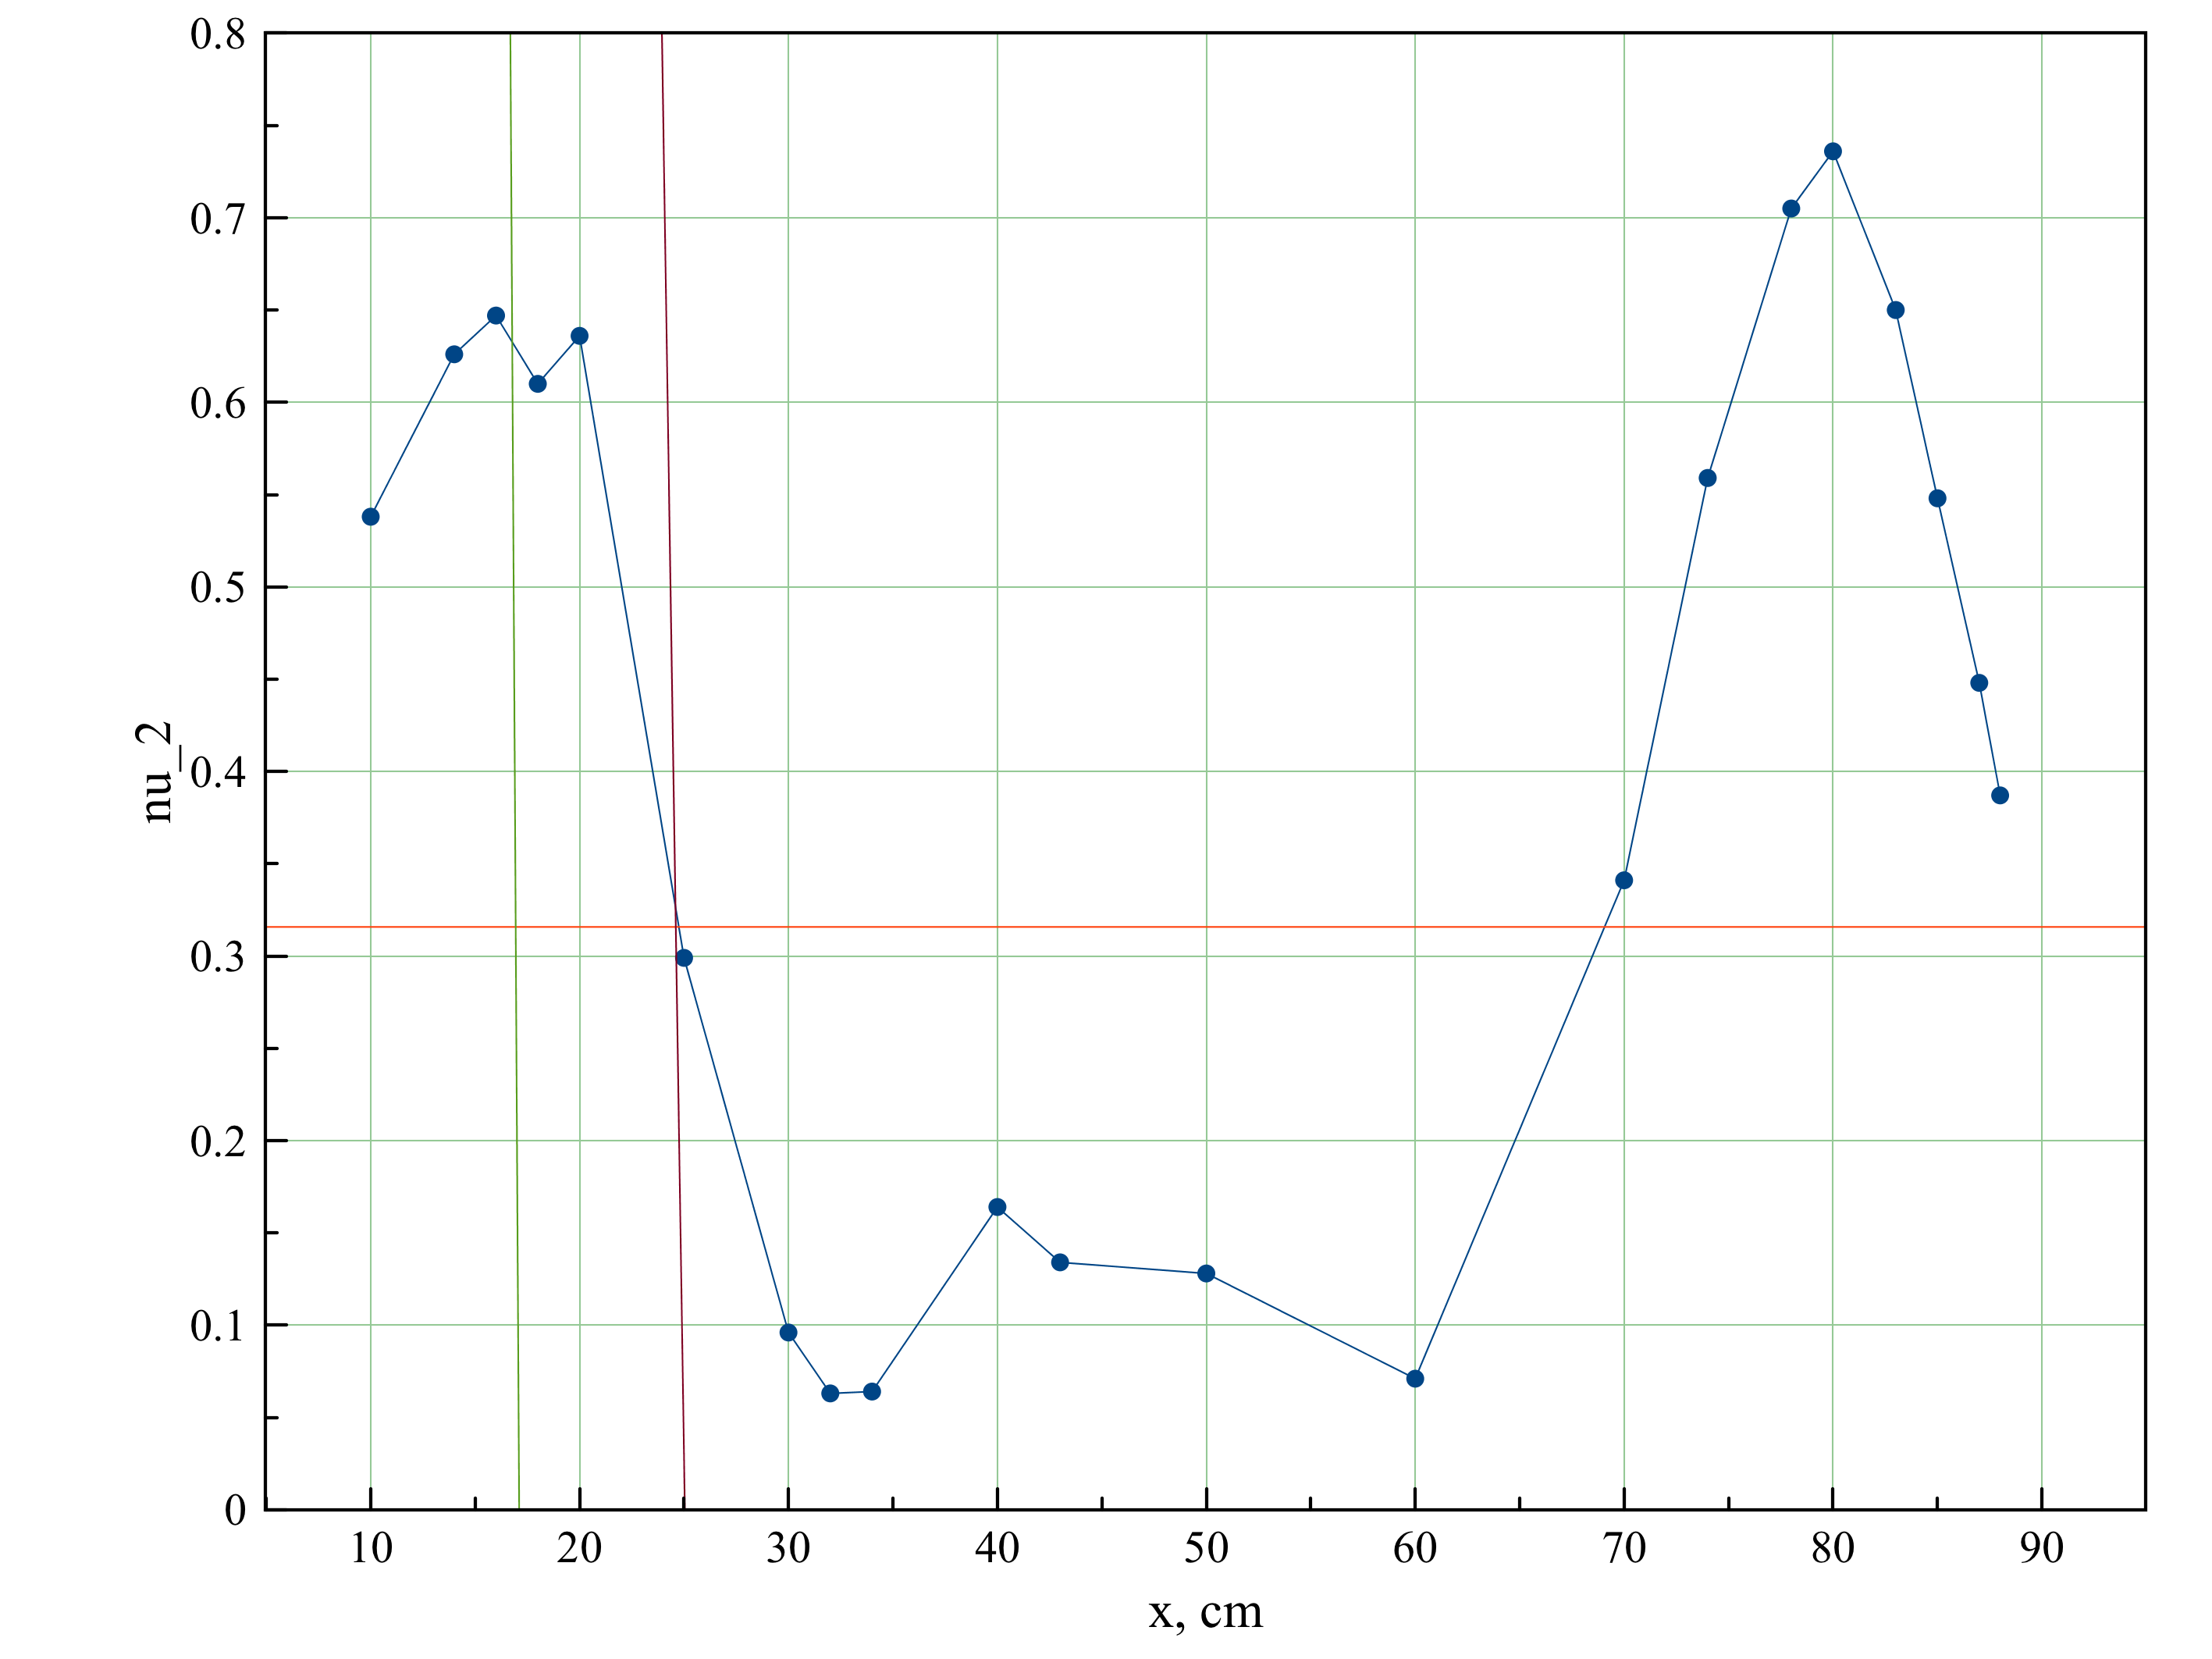
\includegraphics[width = 0.65 \lw]{2.png}
\caption{График зависимости $ \nu_2(x)$}
\end{figure}

По полученному графику определим примерный размер резонатора лазера:
\[ 2L \approx 80 - 16 = 64~\cm \]

Тогда межмодовое расстояние равно:
\[ \Delta \nu_m = \dfrac{c}{2L} = 4,7 \cdot 10^8~\Hz \]

Полуширина первого максимума: 
\[ l_{1/2} = 8~\cm \]

Тогда диапазон частот, в котором происходит генерация продольных мод оценивается выражением:
\[\Delta F = \dfrac{\sqrt{\ln 2} \cdot c}{\pi\cdot l_{1/2}} = 9,9 \cdot 10^8~\Hz \]

Оценим число генерируемых лазером продольных мод:
\[ n \approx 1 + 1.2\dfrac{L}{l_{1/2}} = 6 \]

\section{Вывод}
Исследуя видность интерференционной картины излучения гелий-неонового лазера мы измерили диапазон частот, в котором происходит генерация продольных мод, число продольных мод. Почти точно определили размер резонатора. Зависимость $\nu_2({\cos}^2) \beta$ оказалась линейной, но не проходящей через через ноль (поляроид не перекрывал свет полностью).
\end{document}
